\documentclass[a4paper,12pt]{article}
\usepackage[dutch]{babel}
\usepackage{graphicx}
\usepackage{float}
\usepackage{multicol}

\usepackage{hyperref}
\usepackage{booktabs}
\usepackage{hyphenat}

\usepackage{url} % voor het netjes zetten van URL's
\usepackage{hyperref} % voor hyperlinks
\usepackage{apacite} % extra opties voor citeren met auteur en jaar
\usepackage{graphicx} % voor het opnemen van PDF-, JPG- of PNG-plaatjes
\pagestyle{headings} % zet kopteksten aan
\begin{document}
\title{Een persoonlijk verslag naar de afhandeling van beoordelingssystemiek in geavanceerde algoritmen}
\author{Galvin Bartes}
\maketitle
\begin{abstract} % samenvatting
Een goed rapport heeft een korte en duidelijke samenvatting, die op zichzelf kan staan en niet verwijst naar de rest van het rapport of naar literatuur. De samenvatting is niet te lang maar bevat wel alle belangrijke zaken van het adviesrapport: wat was de vraag, hoe is die beantwoord en wat is de conclusie.
\end{abstract}
\tableofcontents





\newpage
\section{Inleiding\dots}

\newpage
\section{probleemstelling\dots}

\newpage
\section{Scenario}

Uitgaande van het scenario



\begin{table}[hbt!] % drijvende tabel
\caption{States voor Uppaal model.} % bijschrift, wordt automatisch genummerd
\label{reqs} % label om naar figuur te verwijzen
\begin{center} % centreer de tabel
\begin{tabular}{llc} % 3 kolommen, 2 links uitgelijnd en 1 gecentreerd
\hline % horizontale lijn
\textbf{Nr.} & \textbf{Item} & \\ % kolommen gescheiden met &
\hline
1 & Schip A komt aan van links en communiceert met Sluis & \\
1b) & Schip B komt aan van rechts en cmmuniceert met Sluis & \\
aanname & Sluis is leeg & \\
aanname & sluisdeuren 1,2,3,4 zijn dicht & \\
2) & kade stuurt signal naar schip A, mag komen & \\
3) & Schip A komt aan & \\
4) & Kade stuurt signal naar schip B, schip B moet wachten & \\
5) & Schip B gaat afremmen & \\
6) & Schip B is afgeremd voor deur 3 & \\
7) & Schip A krijgt signal sluis deur 1 en 2 gaan open & \\
8) & sluis deur 1 en 2 zijn geopend & \\
9) & Schip A in sluis, sluis A moet afremmen & \\
10) & Schip A gestopt bij ingang van deur drie & \\
11) & Deuren 1 en 2 sluiten & \\
12) & Deuren 1 en 2 gesloten & \\
13) & Nog ruimte voor nog een ship, kade signaleert schip B voor deur 4 & \\
14) & Deur 4 gaat open & \\
15) & deur 4 is geopend & \\
16) & Schip B start op geeft gas, stuurt bij en kiest deur & \\
17) & Schip B afremmen & \\
18) & Schip B gestopt & \\

19) & Sluisdeur sluiten & \\
20) & Sluisdeur gesloten & \\
21) & Sensor aan & \\
22) & sensor geeft hoogte water door aan kade & \\
23) & controller stelt gewenste hoogte voor water bij & \\
24) & pomp activeren & \\
25) & pomp geactiveerd & \\
26) & Sensor hoogte water meten & \\
27) & Water hoogte gemeten & \\
aanname: & eerste keer meten is succesvol & \\
28) &  Sluisdeuren mogen open & \\
29) &  Sluisdeur 2 en 3 zijn geopend & \\
30) &  Schip A en B opstarten & \\
31) & Schip A en B opgestart en rijden weg, verdwijnen uit model & \\
32) & Volgende Schip uit wachtrij wordt in model gebracht & \\
33)  & Kost weinig & \\

\hline
\end{tabular}
\end{center}
\end{table}



\clearpage
\newpage
\section{Excerpt 1}
De rol van functionele eisen


\begin{itemize}
  \item Functionele eis definities:

\end{itemize}


Functionele eis definities:
•	Beslissing pad per unieke geïdentificeerde situatie
•	Vastgelegde communicatie van de interactie van een of meerdere actoren met een systeem weergegeven in een duidelijk begrensde situatie
•	Een functionele eis heeft betrekking op een proces dat het systeem moet uitvoeren of informatie die het systeem moet bevatten. Voorbeelden van functionele eisen zijn eisen die stellen dat het systeem de mogelijkheid moet bieden de beschikbare voorraad te doorzoeken of feitelijke of gebudgetteerde uitgaven moet kunnen rapporteren. Functionele eisen komen direct tot uiting in de volgende stappen van het analyseproces (use-cases, procesmodellen, gegevensmodel), aangezien ze de functies beschrijven die het systeem moet bezitten.

\begin{itemize}

  \item Niet-Functionele eisen:
\end{itemize}
Niet functionele eis definities:
•	Niet functionele eisen verwijzen naar gedragseigenschappen die het systeem moet hebben, zoals goede prestaties en gebruikersvriendelijkheid. De mogelijkheid om via een webbrowser met het systeem te kunnenwerken wordt als een niet-functionele eisen beschouwd. Niet-functionele eisen kunnen de overige sub fasen van het analyseproces (use-cases, procesmodellen en gegevensmode maken) beïnvloeden, maar doe dat vaak slechts indirect. Niet functionele eisen spelen hoofdzakelijk een rol tijdens de ontwerpfase wanneer over de user interfase, de hardware, de software en de onderliggende systeemarchitectuur wordt beslist.





\clearpage
\newpage
\section{Uitwerking casus}

Voor de utiwerking van het model heb ik templates gebruikt die al beschikbaar zijn als demo in Uppaal of uit de selectie van papers.



\begin{itemize}
  \item Nivellerern aangepast iteratiefout:
  \item Sluisdeueren geven deadlock
  \item Reset na final close geeft deadlock
  \item [Entering, adjust_level, stop, start_niveau,] closed geeft deadlock
  \item Verwijderen states Entering, set_level en Restart
  \item Nivellerern aangepast loop verwijderd:
  \item bool Reopendoors geeft deadlock omdat bool moet zijn "&&"en niet '||'

  

\end{itemize}


\begin{table}[hbt!] % drijvende tabel
\caption{Queries voor Uppaal model.} % bijschrift, wordt automatisch genummerd
\label{reqs} % label om naar figuur te verwijzen
\begin{center} % centreer de tabel
\begin{tabular}{llc} % 3 kolommen, 2 links uitgelijnd en 1 gecentreerd
\hline % horizontale lijn
\textbf{Nr} & \textbf{Query} &  \textbf{Result} &\\ % kolommen gescheiden met &
1) & A[] not deadlock & Property is not satisfied & \\
2) & E\<\>\ Schip_l(0).Cross1 and Sluisdeur_l.Closed & \\
3) & A\[\] not (Schip_l(0).Cross2 && not (Sluisdeur_l.Open || Sluisdeur_r.Closed || nivelleer.Nivelleren || Sluisdeur_r.Open || Sluisdeur_l.Closed || Schip_l(1).Safe)) & \\
\hline



\hline
\end{tabular}
\end{center}
\end{table}

\ref{figuur_1}
Random citation \cite{Nobody06} embeddeed in text.




\begin{figure}[hbt!]
    \centering
    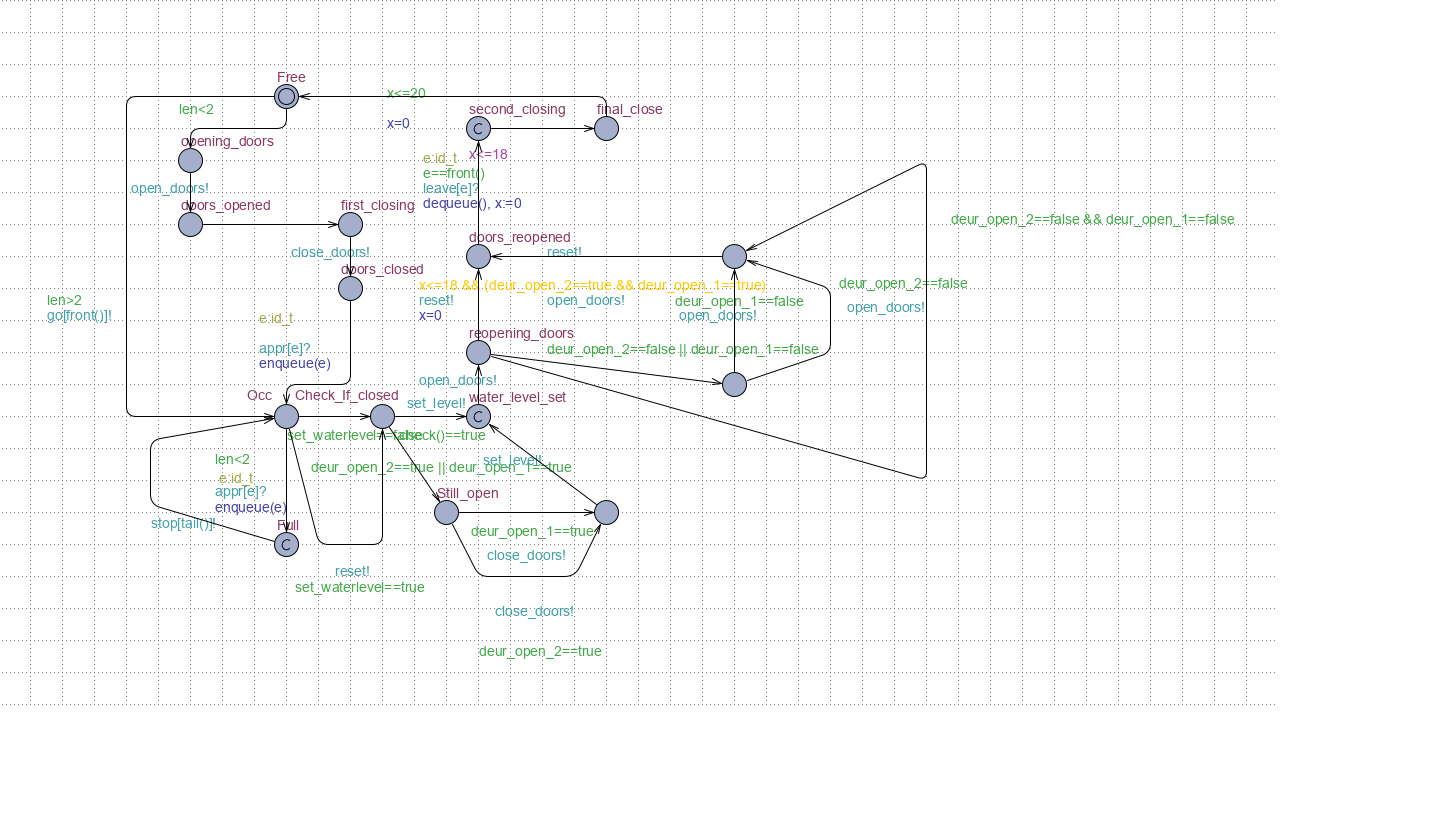
\includegraphics[width=1.0\textwidth]{Controller.png}
    \caption{Controller}
    \label{fig:figuur_1}
\end{figure}


\begin{figure}[hbt!]
    \centering
    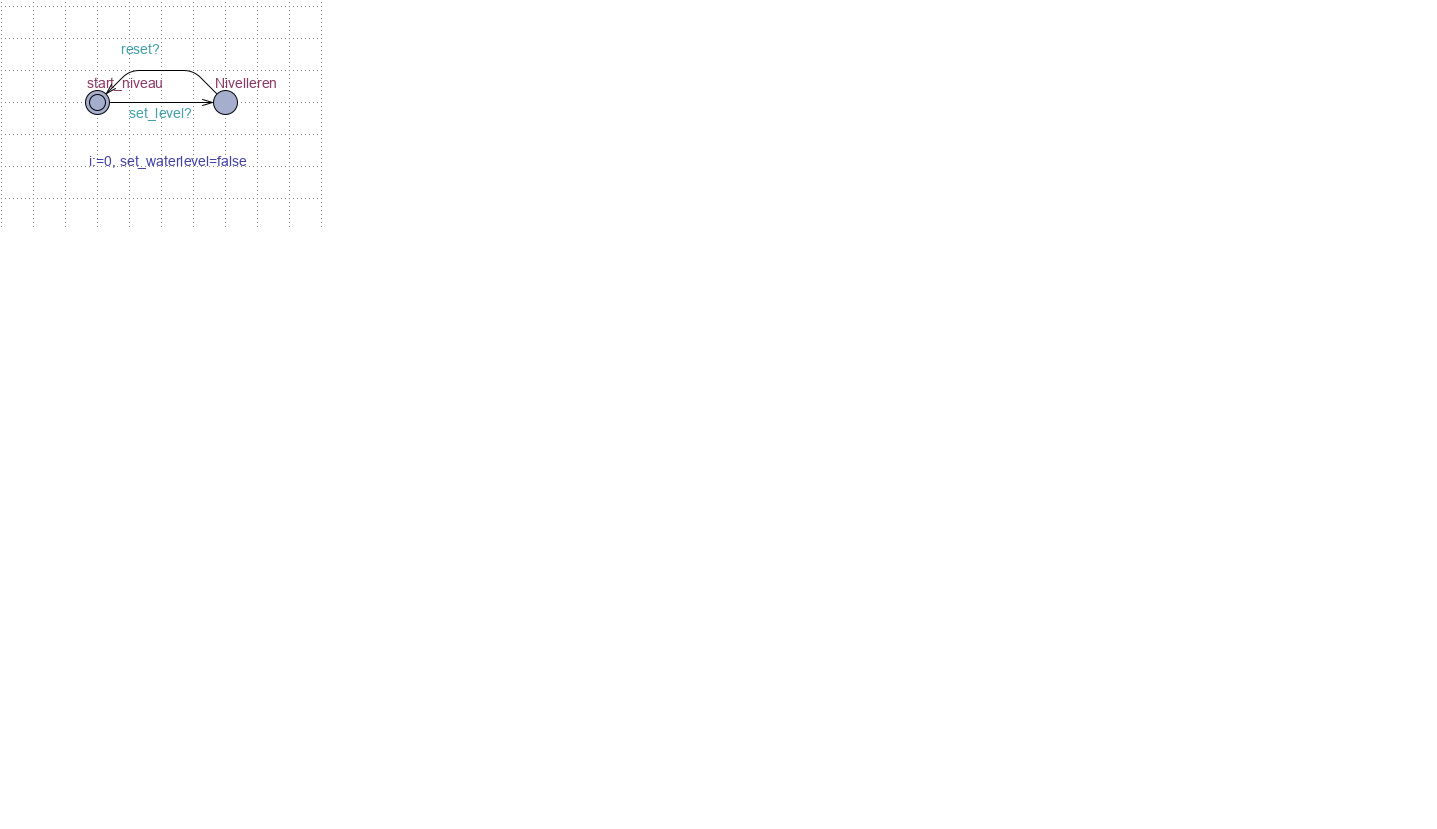
\includegraphics[width=1.0\textwidth]{nivelleer_nieuw.png}
    \caption{nivelleer}
    \label{fig:figuur_2}
\end{figure}



\clearpage
\newpage
\section{Research\dots}



\newpage
\section{Conclusion\dots}

\newpage
\section{Future work\dots}
\begin{itemize}
\item Doe het niet, het is het niet waard.
\item Als je er toch over denkt om het te doen: doe het niet.
\item Kun je het echt niet laten, doe het dan maar.
\end{itemize}
\bibliographystyle{apacite} % literatuurlijst in APA-stijl
\bibliography{literatuurlijst} % neem literatuur op uit bestand literatuurlijst.bib
\end{document}


